\NeedsTeXFormat{LaTeX2e}
%\PassOptionsToClass{handout}{beamer}
\documentclass{beamer}
\usepackage{beamerPack}
\usepackage{setspace}
\usepackage[06]{../lecture}
\subtitle{動的計画法}
\begin{document}

\begin{frame}[fragile]{}
\titlepage
\end{frame}

\section{Dynamic programming and Memoization}		%%%%%%%%
\subsection{}

\begin{frame}[fragile]{アルゴリズムの精錬}{}
\begin{itemize}\itemsep10pt
\item 目的を達成しない(間違った)アルゴリズム
\item 計算量に問題のあるアルゴリズム
\begin{itemize}\itemsep8pt
\item 時間計算量を改善する必要があるアルゴリズム
\begin{quote}
無駄の存在 $\to$ 無駄を省く技術
\end{quote}
\item 空間計算量を改善する必要があるアルゴリズム
\begin{quote}
クイックソートで使用したpartitionは元々は一つの配列から二つの配列に要素をコピー(移動)させるアルゴリズムだったが、改善の結果、あのようなプログラム定義になった
\end{quote}
\end{itemize}
\item 時間的空間的制約も含めて目的を達成するアルゴリズム
\end{itemize}
\end{frame}

\begin{frame}[fragile]{動的計画法}{}
動的計画法は具体的なアルゴリズムではなく、目的を達成するアルゴリズムを生み出すフレームワーク
\vfill
\begin{block}{動的計画法(dynamic programming)}
\begin{itemize}%\itemsep8pt
\item 再帰的に分割された部分問題の(最適)解から元問題の(最適)解を構成
\item 部分問題の重複性の利用
\end{itemize}
\end{block}
\vfill
重複性をどう利用するのか $\to$ 重複しないようにする
\vfill
{\fontsize{8}{9}\selectfont 線形計画法は不等式に関する問題}
\end{frame}

\begin{frame}[fragile]{動的計画法で改善できる例}{}
重複性の利用方法を二つ紹介
\vfill
\begin{itemize}\itemsep8pt
\item
Pascalの三角形 $\to$ 方法1で改善
\item
フィボナッチ数 $\to$ 方法1で改善
\item
素数$\to$ 方法2で改善
\end{itemize}
\vfill
\end{frame}

\begin{frame}[fragile]{Pascalの三角形}{}
\begin{center}
\scalebox{0.6}{
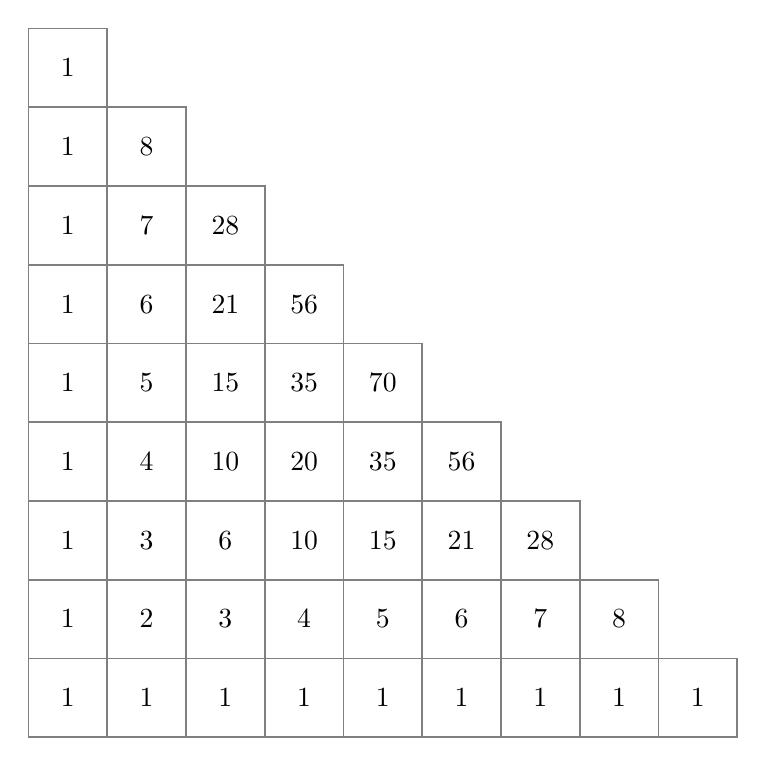
\begin{tikzpicture}[cell/.style = {rectangle,draw=gray,semithick,minimum size=1.0cm,outer sep=0mm}]
\foreach \i [count=\j from 0] in {1, 1, 1, 1, 1,  1, 1, 1, 1}
    \node[cell] at (\j, 0) {\rotatebox{0}{$\i$}};
\foreach \i [count=\j from 0] in {1, 2, 3, 4, 5,  6, 7, 8}
    \node[cell] at (\j, 1) {\rotatebox{0}{$\i$}};
\foreach \i [count=\j from 0] in {1, 3, 6, 10,15,21,28}
    \node[cell] at (\j, 2) {\rotatebox{0}{$\i$}};
\foreach \i [count=\j from 0] in {1, 4, 10,20,35,56}
    \node[cell] at (\j, 3) {\rotatebox{0}{$\i$}};
\foreach \i [count=\j from 0] in {1, 5, 15,35,70}
    \node[cell] at (\j, 4) {\rotatebox{0}{$\i$}};
\foreach \i [count=\j from 0] in {1, 6, 21,56}
    \node[cell] at (\j, 5) {\rotatebox{0}{$\i$}};
\foreach \i [count=\j from 0] in {1, 7, 28}
    \node[cell] at (\j, 6) {\rotatebox{0}{$\i$}};
\foreach \i [count=\j from 0] in {1, 8}
    \node[cell] at (\j, 7) {\rotatebox{0}{$\i$}};
\foreach \i [count=\j from 0] in {1}
    \node[cell] at (\j, 8) {\rotatebox{0}{$\i$}};
\end{tikzpicture}
}
\end{center}
\end{frame}

\begin{frame}[fragile]{Pascalの三角形}{値と実行回数}
\begin{center}
\scalebox{0.6}{
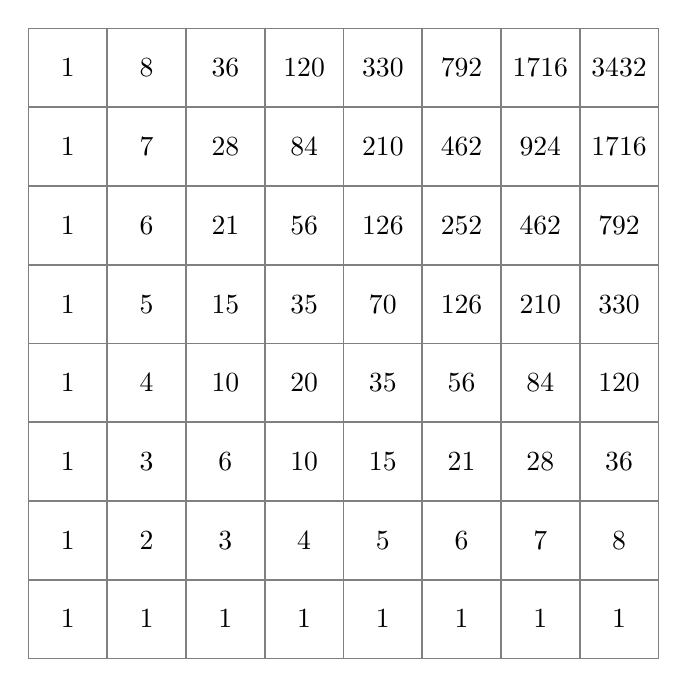
\begin{tikzpicture}[cell/.style = {rectangle,draw=gray,semithick,minimum size=1.0cm,outer sep=0mm}]
\foreach \i [count=\j from 0] in {     1,      1,      1,      1,      1,      1,      1,      1}
    \node[cell] at (\j, 0) {\rotatebox{0}{$\i$}};
\foreach \i [count=\j from 0] in {     1,      2,      3,      4,      5,      6,      7,      8}
    \node[cell] at (\j, 1) {\rotatebox{0}{$\i$}};
\foreach \i [count=\j from 0] in {     1,      3,      6,     10,     15,     21,     28,     36}
    \node[cell] at (\j, 2) {\rotatebox{0}{$\i$}};
\foreach \i [count=\j from 0] in {     1,      4,     10,     20,     35,     56,     84,    120}
    \node[cell] at (\j, 3) {\rotatebox{0}{$\i$}};
\foreach \i [count=\j from 0] in {     1,      5,     15,     35,     70,    126,    210,    330}
    \node[cell] at (\j, 4) {\rotatebox{0}{$\i$}};
\foreach \i [count=\j from 0] in {     1,      6,     21,     56,    126,    252,    462,    792}
    \node[cell] at (\j, 5) {\rotatebox{0}{$\i$}};
\foreach \i [count=\j from 0] in {     1,      7,     28,     84,    210,    462,    924,   1716}
    \node[cell] at (\j, 6) {\rotatebox{0}{$\i$}};
\foreach \i [count=\j from 0] in {     1,      8,     36,    120,    330,    792,   1716,   3432}
    \node[cell] at (\j, 7) {\rotatebox{0}{$\i$}};
\end{tikzpicture}
}
\scalebox{0.6}{
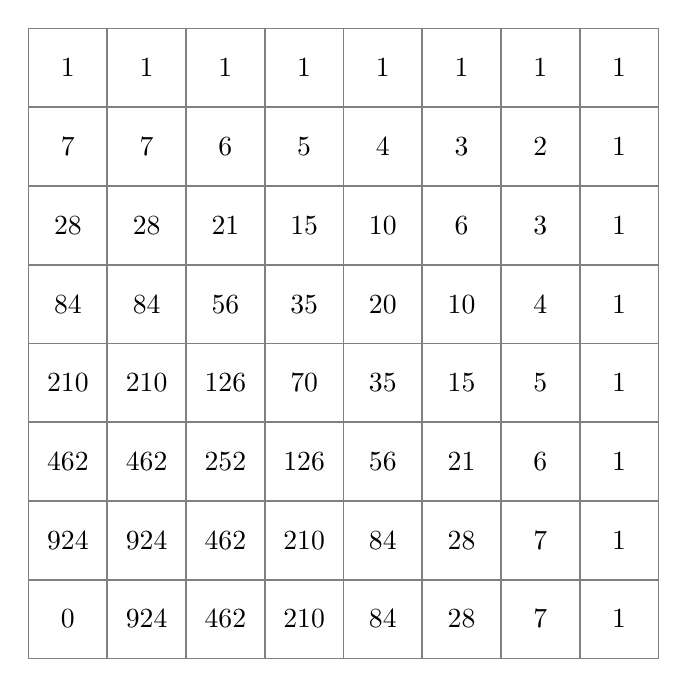
\begin{tikzpicture}[cell/.style = {rectangle,draw=gray,semithick,minimum size=1.0cm,outer sep=0mm}]
\foreach \i [count=\j from 0] in {    0,   924,   462,   210,    84,    28,     7,     1}
    \node[cell] at (\j, 0) {\rotatebox{0}{$\i$}};
\foreach \i [count=\j from 0] in {  924,   924,   462,   210,    84,    28,     7,     1}
    \node[cell] at (\j, 1) {\rotatebox{0}{$\i$}};
\foreach \i [count=\j from 0] in {  462,   462,   252,   126,    56,    21,     6,     1}
    \node[cell] at (\j, 2) {\rotatebox{0}{$\i$}};
\foreach \i [count=\j from 0] in {  210,   210,   126,    70,    35,    15,     5,     1}
    \node[cell] at (\j, 3) {\rotatebox{0}{$\i$}};
\foreach \i [count=\j from 0] in {   84,    84,    56,    35,    20,    10,     4,     1}
    \node[cell] at (\j, 4) {\rotatebox{0}{$\i$}};
\foreach \i [count=\j from 0] in {   28,    28,    21,    15,    10,     6,     3,     1}
    \node[cell] at (\j, 5) {\rotatebox{0}{$\i$}};
\foreach \i [count=\j from 0] in {    7,     7,     6,     5,     4,     3,     2,     1}
    \node[cell] at (\j, 6) {\rotatebox{0}{$\i$}};
\foreach \i [count=\j from 0] in {    1,     1,     1,     1,     1,     1,     1,     1}
    \node[cell] at (\j, 7) {\rotatebox{0}{$\i$}};
\end{tikzpicture}
}
\end{center}
\end{frame}

\begin{frame}[fragile]{重複性の利用方法1:メモ化}{memoization}
計算結果をメモ:2度目からはメモした値をreturn
\vfill
\begin{codeof}{language=}{一般形}
関数(引数) -> 返値 {
  if memoに登録済み { return 登録された値; }
  result = 本来の計算;
  memoにresultを登録
  return result;
}
\end{codeof}
\vfill
動的計画法において部分問題の重複性の改善のために多用される

時間計算量は改善するが空間計算量は増加
\end{frame}

\begin{frame}[fragile]{フィボナッチ数のメモ化$+\alpha$}{}
全く同じ:
\begin{itemize}%\itemsep8pt
\item Pascal:2引数なので(j, i)でメモ
\item Fib: 1引数なのでnでメモ
\end{itemize}
\vfill
ところがメモ化したものがさらに高速化できる
\begin{itemize}%\itemsep8pt
\item メモする範囲の縮退
\end{itemize}
\end{frame}

\begin{frame}[fragile]{重複性の利用方法2:そもそも計算しない}{}
\begin{itemize}\itemsep8pt
\item Pascalの三角形:まだ無駄がある
\item 素数
\item フィボナッチ数(ある意味では)
\end{itemize}
\end{frame}

\begin{frame}[fragile]{計算しない例:素数}{}
自然数$n$が2から$n-1$で割り切れない時、$n$を素数であるという。
\[
\forall k \in [2, n-1] : n \% k \ne 0.
\]

\begin{codeof}{language=Rust}{2からn-1まで割ってみる}
fn is_prime(n: usize) -> bool {
    for i in 2..=n-1 {
        if n % i == 0 { return false; } 
    }
    true
}
\end{codeof}

無駄が存在:小さい数と大きい数のペア:
$
O(n) \to O(\sqrt{n})
$
\end{frame}

\begin{frame}[fragile]{無駄の削除2:そもそも計算しない}{数学的理解でそもそも計算しない}

\[
Fib(n) = \frac{1}{\sqrt{5}}
\left\{
\left(\frac{1 + \sqrt{5}}{2}\right)^n
-
\left(\frac{1 - \sqrt{5}}{2}\right)^n
\right\}
\]

\vfill
\begin{itemize}%\itemsep8pt
\item 指数計算は$\log(n)$のコスト
\item 誤差がある計算
\end{itemize}

\end{frame}

\begin{frame}[fragile]{余談:ふかしぎ おねえさん}{}
数学だけが貢献できるわけではない。場合によってはプログラミング技術(計算機科学)が大きな貢献をすることもある:YouTubeで ふかしぎ おねえさん を検索

\vfill
\begin{itemize}%\itemsep8pt
\item メインテーマは簡単そうに見えてすごい問題があること(アルゴリズムの話ではない)
\item 簡単そうに見えて数学者が一般項を発見できてない
\item 使えるアルゴリズムは数え上げという原始的な方法のみ
\item エンディング中に数え上げで使うデータ構造の改良を紹介
\item \textit{The Art of Comp. Prog.}に紹介(絶賛)された、数少ない日本人による成果
\end{itemize}
\end{frame}

\begin{frame}[fragile]{そもそも計算しない関連の余談}{}

\begin{codeof}{language=Rust}{これはコンパイラが対応してくれるか?}
if f(x) == 0 {
  ...
}
else if f(x) != 0 {
  ...
}
\end{codeof}

\begin{codeof}{language=Rust}{}
if p(x) == true {
  return true;
}
else {
  return false
}
\end{codeof}

return p(x);
\end{frame}

\section{Extra puzzles}		%%%%%%%%
\subsection{}

\begin{frame}[fragile]{時間が余るなら}{Advent of Code: year 2020, day 10}
\begin{enumerate}\itemsep8pt
\item 与えられた数列は以下の条件を満たす数列に変換できるか
\begin{itemize}%\itemsep8pt
\item 全ての項は、直前の項より1、2、または3大きい
\end{itemize}
\begin{enumerate}%\itemsep8pt
\item 数列1:\{ 16, 10, 15, 5, 1, 11, 7, 19, 6, 12, 4 \}
\item 数列2:もっと長い(91項)ので次ページに掲載
\end{enumerate}
\item 所与の数列に対し以下の条件を満たす数列の個数を求めよ
\begin{itemize}%\itemsep8pt
\item その列中の全ての項は、直前の項より1、2、または3大きい
\item 与えられた全ての項を使わなくてよい
\item ただし、所与の数列の最小項は必ず使うこと
\item ただし、所与の数列の最大項は必ず使うこと
\end{itemize}
\begin{enumerate}%\itemsep8pt
\item 先の数列1
\begin{enumerate}%\itemsep8pt
\item 求める数列は1で始まらなければならない
\item 求める数列は19で終わらなければならない
\item 例えば\{ 1, 4, 5, 7, 10, 12, 15, 16, 19 \}は条件を満たす
\item 網羅すると8通りあることがわかるので答えは8
\end{enumerate}
\item (64bit CPU所有者のみ)次ページの数列2
\end{enumerate}
\end{enumerate}
\end{frame}

\begin{frame}[fragile]{数列2}{}
95
43
114
118
2
124
120
127
140
21
66
103
102
132
136
93
59
131
32
9
20
141
94
109
143
142
65
73
27
83
133
104
60
110
89
29
78
49
76
16
34
17
105
98
15
106
4
57
1
67
71
14
92
39
68
125
113
115
26
33
61
45
46
11
99
7
25
130
42
3
10
54
44
139
50
8
58
86
64
77
35
79
72
36
80
126
28
123
119
51
22
\end{frame}
\end{document}

\begin{frame}[fragile]{ダイクストラ法}{
%\href{https://ja.wikipedia.org/wiki/ダイクストラ法}{\beamergotobutton{wikipedia}}
}
\begin{quotation}
\fontsize{9}{12}\selectfont
最短経路問題は、ビー玉と紐を用いて解くことができる。
まずビー玉を頂点、紐を辺にするグラフを工作する。
グラフを板の上に置き、スタートの頂点にあたるビー玉だけをつまむ。
グラフが置かれている板を取り除くと、グラフは自由落下を始めるが、スタートにあたるビー玉を持っているので、スタート地点から近いビー玉から順に落下が止まる。
ゴールにあたるビー玉が止まったとき、ゴールにあたるビー玉はスタートにあたるビー玉まで紐で一直線で結ばれている。
この直線が最短経路である。

ダイクストラのアルゴリズムは、上述の解法をコンピュータ上でシミュレートしたものである。
\end{quotation}
\end{frame}

\begin{frame}[fragile]{ダイクストラ法の根幹:相似問題の考え方による説明}{中間目標を設定し相似問題に帰着させたい}
中間目標の選択:どの頂点が確定できるか
\begin{itemize}\itemsep8pt
\item 距離確定頂点から最も「近い」未確定頂点とする
\begin{itemize}%\itemsep8pt
\item なぜならこの頂点に限り三角不等式が成立するから

\begin{center}
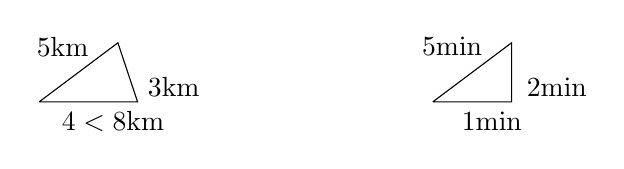
\begin{tikzpicture}[scale=0.25]
\draw (0, 0)
    -- (4, 3) node[near end, above=4pt, anchor=east] {$5$km}
    -- (5, 0) node[near end, right=2pt] {$3$km}
    -- (0, 0) node[near start,below] {$4<8$km};
\draw (20, 0)
    -- (24, 3) node[near end, above=4pt, anchor=east] {$5$min}
    -- (24, 0) node[near end, right=2pt] {$2$min}
    -- (20, 0) node[near start, below] {$1$min};
\end{tikzpicture}
\end{center}

\end{itemize}
\item この選択の余地の少なさが中間目標の変更を要請する
\begin{itemize}%\itemsep8pt
\item これまでの中間目標は終点から;今回は始点から
\end{itemize}
\end{itemize}

\vfill
相似問題:
\begin{itemize}\itemsep8pt
\item 頂点数が1減ったもの
\end{itemize}
\end{frame}
